\clearpage
\section{Methods}
\label{sec:4.4_methods}


% 4.3.1
% -----
\subsection{CLEMnet architecture}
\label{sec:4methods_architecture}

Inspired by the U-net architecture \cite{ronneberger2015u,ounkomol2018label}, the CNN developed for label-free predictions is comprised of a multi-stage contraction path followed by a relatively shorter expansion path. This asymmetry is a result of the resolution difference between EM and FM images. The network is trained on large-scale (exact number of GBs) correlative FM and EM datasets amassed via an integrated array tomography workflow. That is, serial section imaging facilitated by an integrated light and electron microscope \cite{liv2013simultaneous,lane2021optimization}


\subsubsection{Hyperparameter tuning}


\subsubsection{Loss functions}





% 4.3.0
% -----
\subsection{Tissue and sample preparation}
\label{sec:4methods_prep}

\subsubsection{Rat pancreas}
\label{sec:4methods_prep_rp}

\subsubsection{HeLa cells}


% 4.3.2
% -----
\subsection{Data acquisition}
\label{sec:4methods_acquisition}

The integrated microscopy workflow for large-scale correlative imaging and reconstruction is described in \textcite{lane2021optimization}. Briefly, FM imaging is done via the Delmic SECOM (Delmic B.V.), which has been retrofitted into the vacuum chamber of an FEI Verios SEM (Thermo Fisher Scientific) \cite{liv2013simultaneous,zonnevylle2013integration}. FM image tiles are acquired in a grid-like pattern encompassing each tissue section. Each FM image consists of a \SI{10}{\second} exposure at \SI{405}{\nano\meter} excitation for Hoechst and \SI{555}{\nano\meter} excitation for AF594. A low magnification EM image of the same field of view is acquired immediately after each FM acquisition. The EM image is then registered to the FM image by means of cathodoluminescence markers \cite{haring2017automated}. Following the acquisition of the correlative FM--low magnification EM tiles, a grid of high magnification EM tiles is acquired. For the case of the rat pancreas tissue, insulin expression from AF594 guides the acquisition area to islets of Langerhans. As thin sections of the HeLa cells are more or less homogeneous, acquisition areas were chosen based on minimal damage to the section. The exact imaging parameters for high magnification EM acquisitions are presented in Tables \ref{tab:4.1_params_rp} and \ref{tab:4.2_params_zf} for the rat pancreas tissue and HeLa cells respectively.

\begin{table}[tbh]
    \small
    \begin{tabular}
        {r % Z
         r % Section
         >{\raggedleft\arraybackslash}p{1.5cm} % LE
         r % Dwell
         >{\raggedleft\arraybackslash}p{1.5cm} % PS
         >{\raggedleft\arraybackslash}p{1.5cm} % N
         >{\raggedleft\arraybackslash}p{2.5cm} % A
         >{\raggedleft\arraybackslash}p{1.5cm} % T
        }
        \toprule
        Z index & Section & LE (eV) & Dwell (µs) & Pixelsize (nm) & N. EM images & Area (µm × µm) & Acquisition time (hr) \\ 
        \midrule
        1 & S001 & 1500 & 2 & 4 & 169 & 208 × 208 & 1.6 \\
        3 & S003 & 1500 & 2 & 4 & 169 & 208 × 208 & 1.6 \\
        4 & S004 & 1500 & 2 & 4 & 169 & 208 × 208 & 1.6 \\
        7 & S007 & 1500 & 2 & 4 & 169 & 208 × 208 & 1.6 \\
        9 & S009 & 1500 & 2 & 4 & 169 & 208 × 208 & 1.6 \\
        10 & S010 & 1500 & 2 & 4 & 169 & 208 × 208 & 1.6 \\
        \bottomrule
    \end{tabular}
    \caption{
    \textbf{Electron microscopy imaging settings used for the acquisition of rat pancreas tissue. Acquisitions were centered around the islets of Langerhans present in each section.}
    }
    \label{tab:4.1_params_rp}
\end{table}


% Table 4.1 (params)
% ------------------
\begin{table}[tbh]
    \small
    \begin{tabular}
        {r % Z
         r % Section
         >{\raggedleft\arraybackslash}p{1.5cm} % LE
         r % Dwell
         >{\raggedleft\arraybackslash}p{1.5cm} % PS
         >{\raggedleft\arraybackslash}p{1.5cm} % N
         >{\raggedleft\arraybackslash}p{2.5cm} % A
         >{\raggedleft\arraybackslash}p{1.5cm} % T
        }
        \toprule
        Z index & Section & LE (eV) & Dwell (µs) & Pixelsize (nm) & N. EM images & Area (µm × µm) & Acquisition time (hr) \\ 
        \midrule
        \rowcolor{gray!20}
        0 & S002A & 1500 & 3 & 3 & 484 & 234 × 234 & 6.8 \\
        \rowcolor{gray!20}
        1 & S003B & 1500 & 1 & 3 & 484 & 234 × 234 & 2.3 \\
        \rowcolor{gray!20}
        2 & S003C & 1500 & 2 & 3 & 484 & 234 × 234 & 4.5 \\
        \rowcolor{gray!20}
        3 & S003D & 1500 & 2 & 4 & 289 & 241 × 241 & 2.7 \\
        \rowcolor{gray!20}
        4 & S004A & 1500 & 2 & 5 & 196 & 249 × 249 & 1.8 \\
        \rowcolor{gray!20}
        5 & S004B & 1500 & 2 & 6 & 121 & 235 × 235 & 1.1 \\
        \rowcolor{gray!20}
        6 & S005A & 1500 & 5 & 3 & 484 & 234 × 234 & 11.3 \\
        \rowcolor{gray!20}
        7 & S005B & 2000 & 2 & 3 & 484 & 234 × 234 & 4.5 \\
        \rowcolor{gray!20}
        8 & S006A & 1000 & 2 & 3 & 484 & 234 × 234 & 4.5 \\
        \rowcolor{gray!20}
        9 & S006B & 3000 & 2 & 3 & 484 & 234 × 234 & 4.5 \\
        10 & S007A & 1500 & 2 & 3 & 484 & 234 × 234 & 4.5 \\
        11 & S007B & 1500 & 2 & 3 & 484 & 234 × 234 & 4.5 \\
        12 & S008A & 1500 & 2 & 3 & 484 & 234 × 234 & 4.5 \\
        13 & S008B & 1500 & 2 & 3 & 484 & 234 × 234 & 4.5 \\
        14 & S008C & 1500 & 2 & 3 & 484 & 234 × 234 & 4.5 \\
        15 & S008D & 1500 & 2 & 3 & 484 & 234 × 234 & 4.5 \\
        16 & S008E & 1500 & 2 & 3 & 484 & 234 × 234 & 4.5 \\
        17 & S009A & 1500 & 2 & 3 & 484 & 234 × 234 & 4.5 \\
        18 & S009B & 1500 & 2 & 3 & 484 & 234 × 234 & 4.5 \\
        19 & S009C & 1500 & 2 & 3 & 484 & 234 × 234 & 4.5 \\
        \bottomrule
    \end{tabular}
    \caption{
    \textbf{Electron microscopy imaging settings used for the acquisition of resin-embedded HeLa cells.}
    Baseline settings for which all imaging parameters remained constant are highlighted in gray.}
    \label{tab:4.2_params_zf}
\end{table}


\subsubsection{Data availability}
All of the image data used in this work is available at \href{http://nanotomy.org/}{www.nanotomy.org}. Visualization and navigation of large-scale datasets is made possible by CATMAID \cite{saalfeld2009catmaid}.



% 4.3.3
% -----
\subsection{Quantitative analysis}
\label{sec:4methods_analysis}

\subsubsection{Cell nuclei counting}
A combination of experts and trained volunteers were asked to recognize cell nuclei in datasets comprised of true fluorescence and network-generated fluorescence images. The experts consisted of two researchers from the University Medical Center Groningen who routinely examine islets of Langerhans, while the volunteers consisted of thirteen researchers from within the TU Delft Department of Imaging Physics who were trained to recognize cell nuclei in both FM and EM image data from comparable tissue.

An unsupervised, brute-force nearest neighbors search was used to filter outlier annotations from the EM dataset. For each annotated point, the Euclidean distance to every other annotated point was calculated. If a point was found to have at least 12 neighboring points (corresponding to $\ge\SI{80}{\percent}$ of annotators) within a radius roughly equal to the average radius of a cell nucleus, the point was kept. Points with an insufficient amount of neighboring points were discarded, resulting in clusters of point clouds corresponding to the ground truth nuclei. $k$-means clustering was then used to agglomerate point clouds from which the centroid of each cluster could be computed and added to the ground truth set.


\subsubsection{Metrics}

\header{Precision and recall}
Precision and recall are widely used metrics in machine learning and computer vision to assess how successful a model is at certain pattern recognition tasks. In this work the typical object recognition task is reversed as humans are asked to identify objects in images generated by a machine learning model. The same conventions for assessing object recognition nevertheless apply. Provided some object recognition task, precision measures the number of correctly identified objects relative to the amount of objects retrieved by the search, while recall measures the number of correctly identified objects relative to the total amount of objects that ought to have been identified. The number of correctly identified objects are referred to as true positives (TP),
while the number of incorrectly identified objects and missed objects that ought to have been identified are referred to as false positives (FP) and false negatives (FN) respectively, such that
\begin{equation}
    \text{precision} = \frac{TP}{TP+FP}
\end{equation}
%
\begin{equation}
    \text{recall} = \frac{TP}{TP+FN}
\end{equation}
%
The Dice similarity coefficient (alternatively the $F1$ score) combines precision and recall to measure the overall accuracy of a detection system.
\begin{equation}
    F1 = 2\, \frac{Pr \times Re}{Pr+Re}
\end{equation}


\header{PCC}
Network performance is characterized in part by the Pearson correlation coefficient (PCC or $\rho$), a measure of how well two signals ($X$, $Y$) are linearly correlated. It is calculated as the normalized covariance of the two signals.
%
\begin{align}
    \rho &= \frac{\text{cov}(X, Y)}{\sigma_X \sigma_Y} \\
    &= \frac{\sum\left(X_i - X_{avg}\right)
             \sum\left(Y_i - Y_{avg}\right)}
            {\sqrt{\sum\left(X_i - X_{avg}\right)^2}
             \sqrt{\sum\left(Y_i - Y_{avg}\right)^2}}
\end{align}
%

\header{Manders coefficient}
Some stuff about Manders coefficient


\header{Colocalization maps}
Some stuff about colocalization maps


% 4.3.4
% -----
\subsection{Robustness \& validation}
\label{sec:4methods_augment}
Electron and fluorescence microscopy image data is augmented during training to increase the robustness of the model. The idea is more so to improve the model's flexibility and to account for different types of imaging conditions than it is to extend it to different specimens. While the model may generate reasonable predictions of the fluorescence intensity on the same cell type or organelle across different specimens, it is not generalizable to tissue or cell types it has not been trained on. Several different types of data augmentation are applied to account for the variety of imaging settings the network would reasonably encounter if tested on EM data from other instruments.

\subsubsection{Affine transformation}
Affine transformations are applied to training data such that the model learns to adapt to modest changes in structural topology. By introducing minor adjustments to the rotation ($\theta$), translation ($t_x$, $t_y$), scale ($z_x$, $z_y$), and shear ($\Gamma$) of the training data, some degree of invariance to these transformations is embedded into the model \cite{simard2003best}. The applied affine transformations are randomized for each EM-FM image pair such that each image pair receives the exact same transformation (Figure \ref{fig:4m_affine}).

% Mfig 4.? (affine)
% -----------------
\begin{figure}[!tbh]
    \centering
    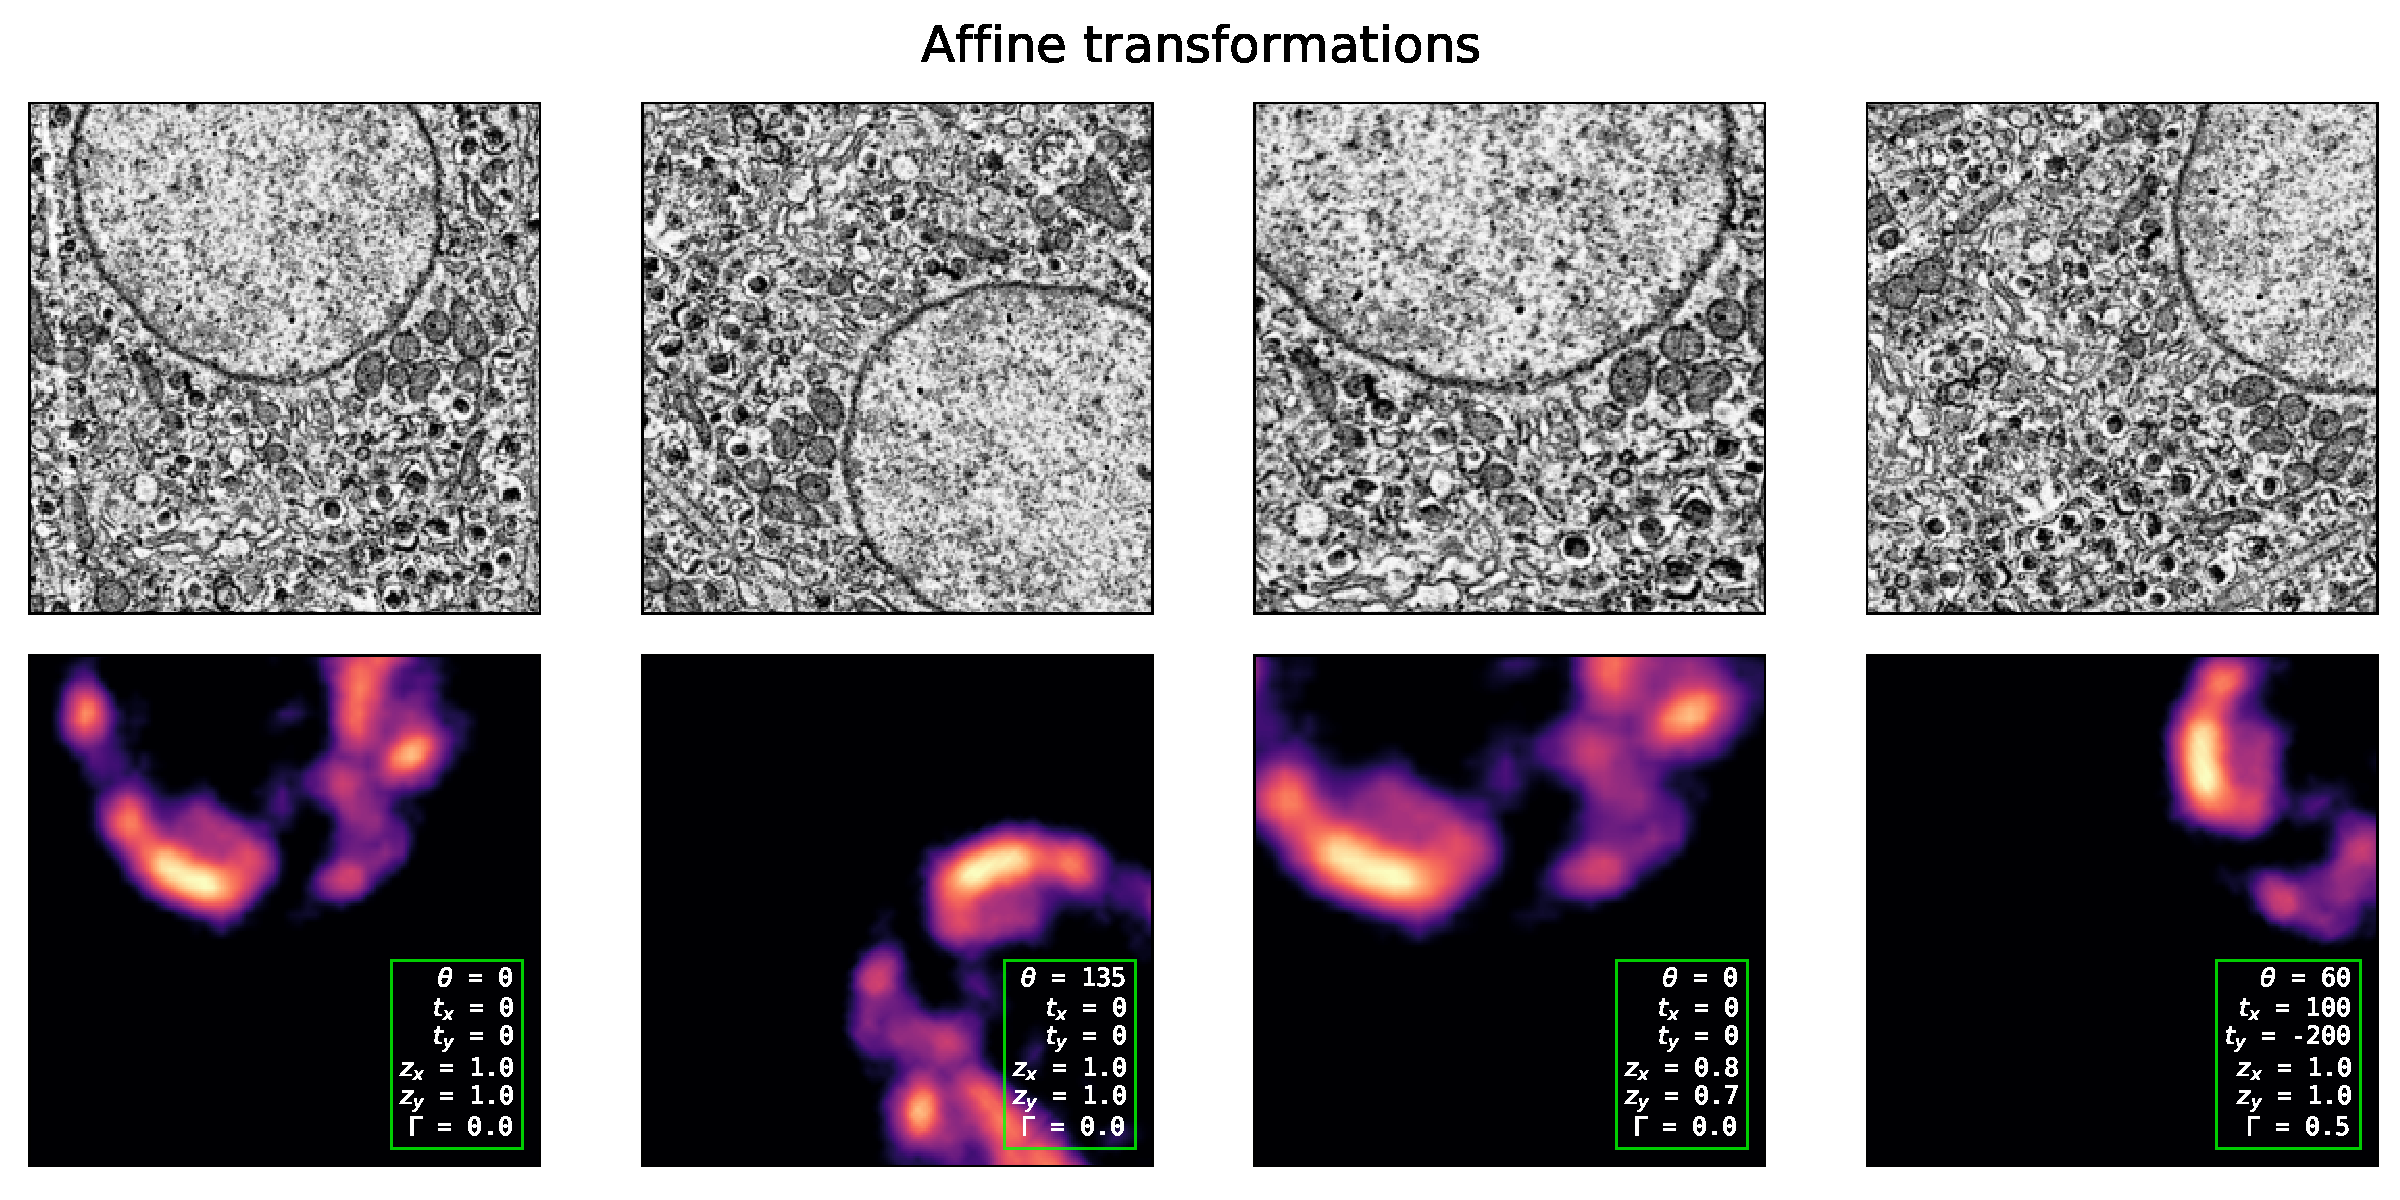
\includegraphics[width=\linewidth]{chapter-4/mfigs/mfig_affine.pdf}
    \caption{\textbf{Affine transformations are applied to the training data to render the model invariant to topological changes, resulting in greater robustness.}
    The original, correlative image pair (left) may be rotated, translated, scaled, and sheared to encompass a wide variety of possible topological changes. Exact transformation parameters are provided in each transformed image.}
    \label{fig:4m_affine}
\end{figure}

\subsubsection{Elastic deformation}
Elastic deformation was identified by \textcite{simard2003best} early in the development of neural networks as an effective means of augmenting training data. It was later shown by \textcite{dosovitskiy2014discriminative} and reinforced by \textcite{ronneberger2015u} as a crucial tool for enhancing CNN training, particularly in the case of limited training samples. Elastic deformations are generated by applying a non-linear warp to the image where the warp is defined by a displacement field convolved with a Gaussian kernel of standard deviation, $\sigma$, and multiplied by a scaling factor, $\alpha$ (Figure \ref{fig:4m_maps}). The displacement field is initialized by a random uniform distribution where each pixel ranges from $(-1, +1)$ with equal probability. The value for $\alpha$ is also randomized such that the EM images are warped with varying intensity; a random uniform distribution from $(1, 3)$ was chosen empirically (Figure \ref{fig:4m_elastic}).

% Mfig 4.? (maps)
% ---------------
\begin{figure}[!tbh]
    \centering
    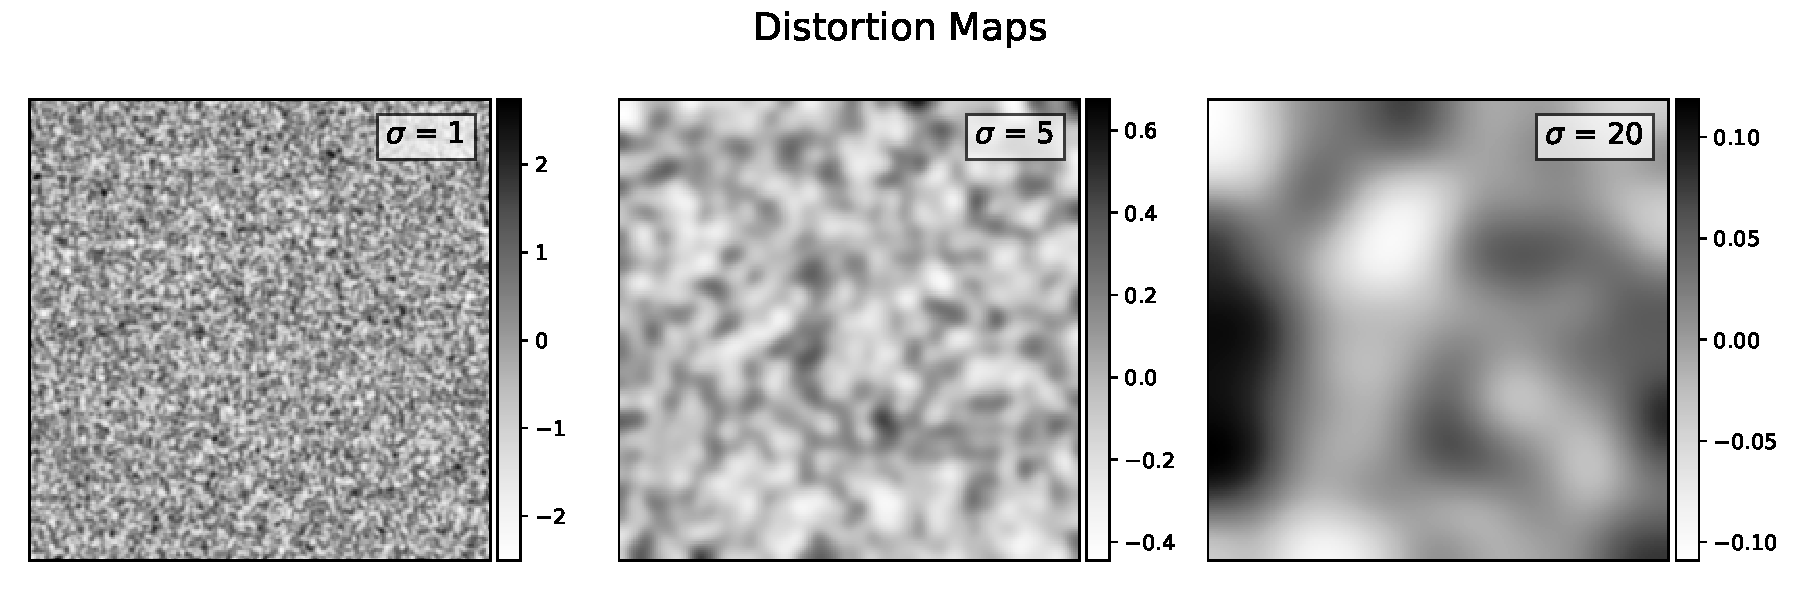
\includegraphics[width=\linewidth]{chapter-4/mfigs/mfig_maps.pdf}
    \caption{\textbf{Deformation maps used for applying elastic deformations to training data.}
    The standard deviation of the Gaussian kernel is varied in each deformation map. For small $\sigma$, the resulting elastic deformation resembles the addition of white noise, while for large $\sigma$, the deformation is quite severe.}
    \label{fig:4m_maps}
\end{figure}

% Mfig 4.? (elastic)
% ------------------
\begin{figure}[!tbh]
    \centering
    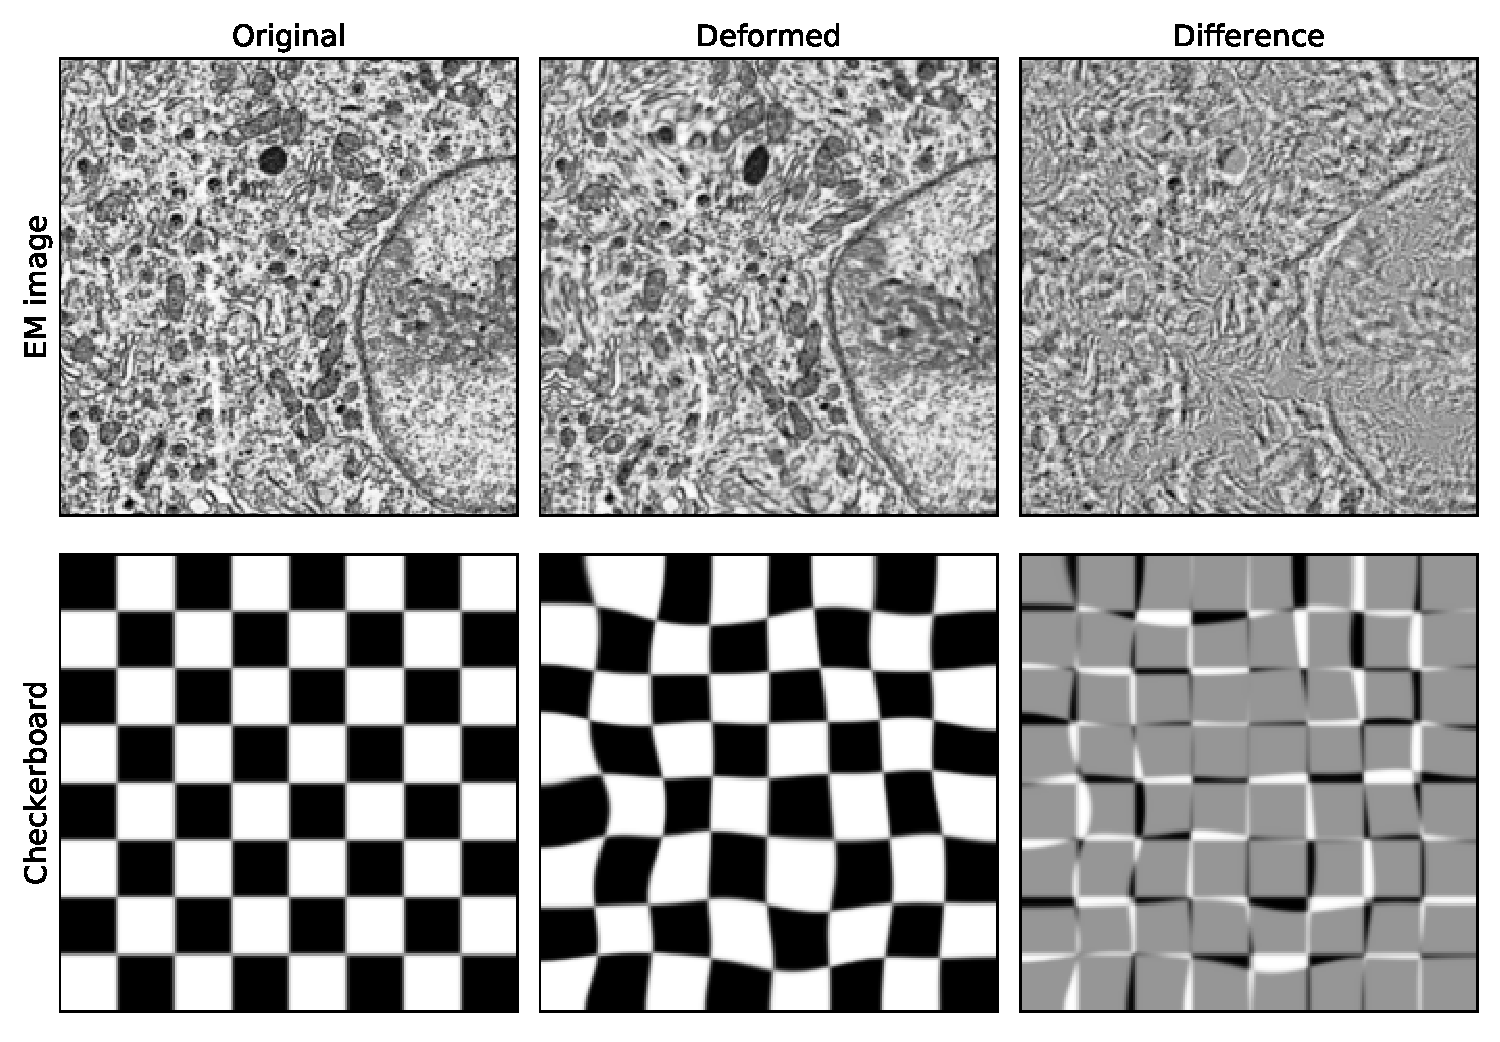
\includegraphics[width=0.9\linewidth]{chapter-4/mfigs/mfig_example.pdf}
    \caption{\textbf{Elastic deformation applied to a typical electron microscopy training image and a checkerboard pattern.}
    Deformation is exaggerated to illustrate the effect of the distortion; $\sigma=20$, $\alpha=400$. The difference images (right) (particularly that of the checkerboard pattern) reveal that while local intensity changes can be quite drastic, the image retains its overall structure.}
    \label{fig:4m_elastic}
\end{figure}

\subsubsection{Brightness \& contrast variation}
To account for the expected variations to brightness and contrast in EM image data acquired across different samples, microscopes, imaging settings, (day of the week), etc. the brightness and contrast levels are given a random adjustment. The brightness is varied $\SI{\pm20}{\percent}$ by adding a gray-level bias, while the contrast is adjusted in the range $(0.75 < \delta < 1.5)$ where the value of each pixel, $x$, is scaled by
%
\begin{equation}
    (x - \bar{x})\,\delta + \bar{x}
\end{equation}
%
where $\bar{x}$ is the average intensity of the whole image.

\subsubsection{Noise augmentation}
Account for noise levels caused by different dwell times and detector types and quality. Poisson noise example. (Figure \ref{fig:4m_noise}). Some shot noise theory.
%
\begin{equation}
    f(k;\lambda) = \frac{\lambda^{k} e^{-\lambda}}{k!}
\end{equation}

% Mfig 4.? (noise)
% ----------------
\begin{figure}[!tbh]
    \centering
    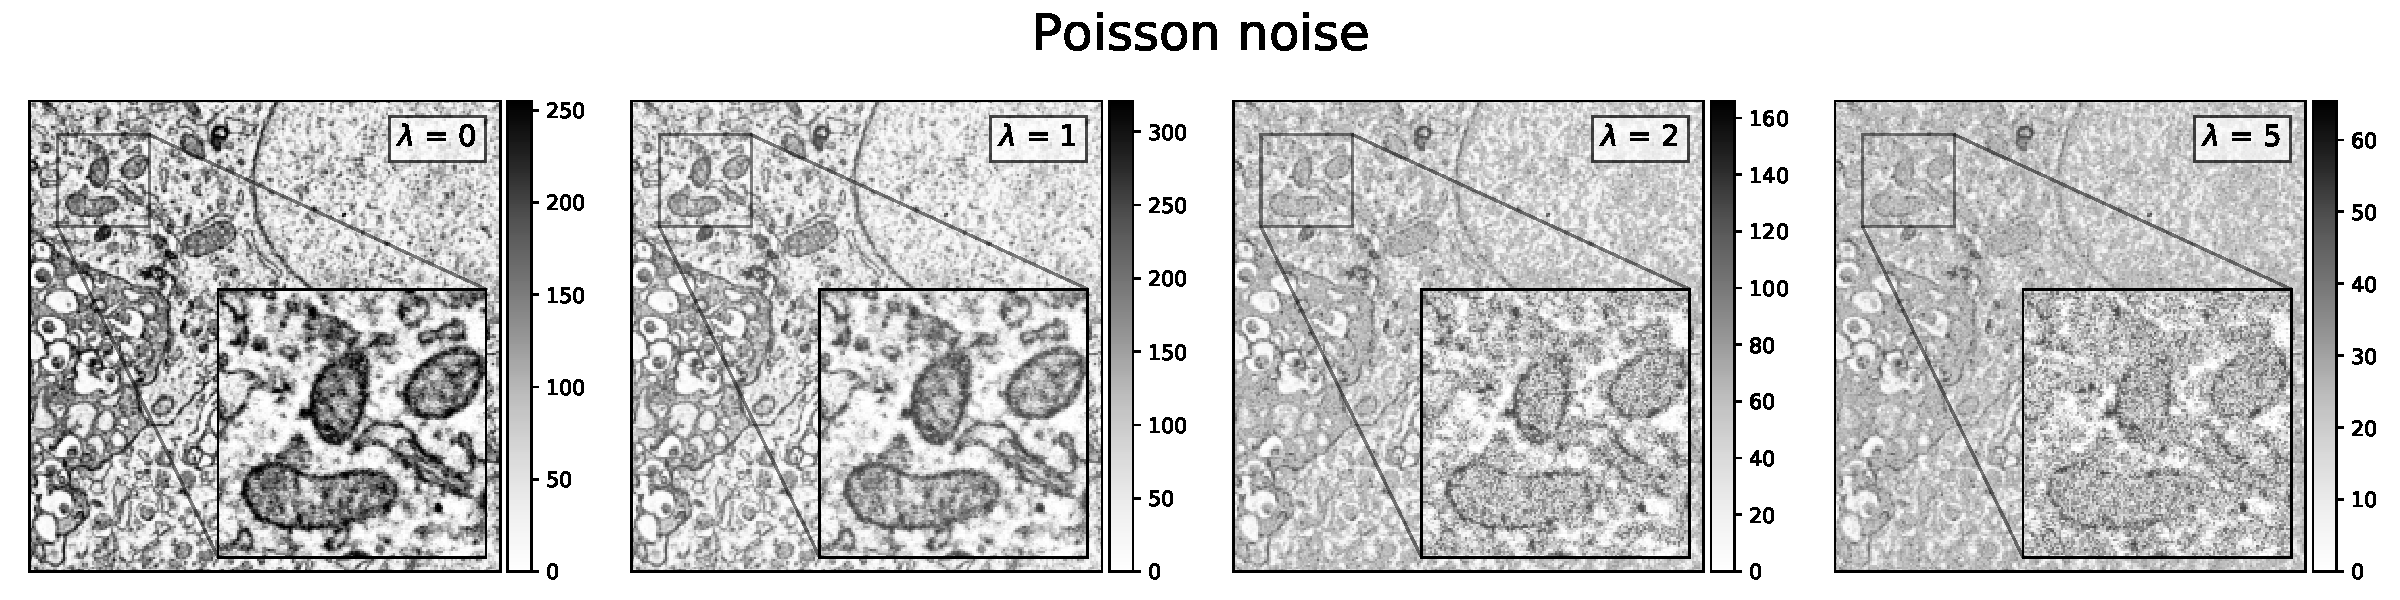
\includegraphics[width=\linewidth]{chapter-4/mfigs/mfig_noise.pdf}
    \caption{\textbf{Poisson noise.}
    Caption.}
    \label{fig:4m_noise}
\end{figure}


% 4.4.6 Segmentation
% ------------------
\subsection{Segmentation}
\label{sec:4methods_segmentation}

\subsubsection{[Fully supervised] segmentation}


\subsubsection{Partial points segmentation}
% mask image is created, mostly unlabelled
% Pixels are classified as either nucleus, background, or unlabelled according to the criteria
% \begin{equation}
%     L = \begin{cases}
%     0 & \text{if} 0 \\
%     \end{cases}
% \end{equation}

% \begin{cases}
%       M_i & \text{if}\; D_i < r_2, \\
%       0 & \text{if}\; D_i > r_2 \;\text{and}\; (p_i < 0.1 \;\text{or}\; p_i > 0.7), \\
%       -1 & \text{otherwise}
%     \end{cases}
% self training to refine nuclei detection

% labels are merged
% self-training
